\chapter{Grundlagen}
\label{chapter:grundlagen}

In diesem Kapitel werden die für diese Arbeit relevanten theoretischen und konzeptuellen Grundlagen beschrieben. Begonnen wird mit einer kurzen Einführung in das Brettspiel Patchwork. Anschließend widmet sich dieses Kapitel der Spieltheorie, einem mathematischen Bereich, der bei der Modellierung und Analyse von Entscheidungssituation verwendet wird. Dann wird der Minimax-Algorithmus betrachtet, der den grundlegenden Algorithmus für einen in dieser Arbeit implementierten Computergegner darstellt. Anschließend werden die Grundlagen für zwei weitere Computergegner geschaffen, indem die Theorie von \acl{MCTS} und AlphaZero erläutert wird. Abschließend werden interaktive System erläutert, die für die Gestaltung der Benutzerschnittstellen und Spielererfahrung der Computerumsetzung des Brettspiels wichtig sind.

\section{Brettspiel Patchwork}
\label{chapter:brettspiel-patchwork}

\begin{wrapfigure}{r}{0.325\textwidth}
    \centering
    \vspace*{-0.75cm}
    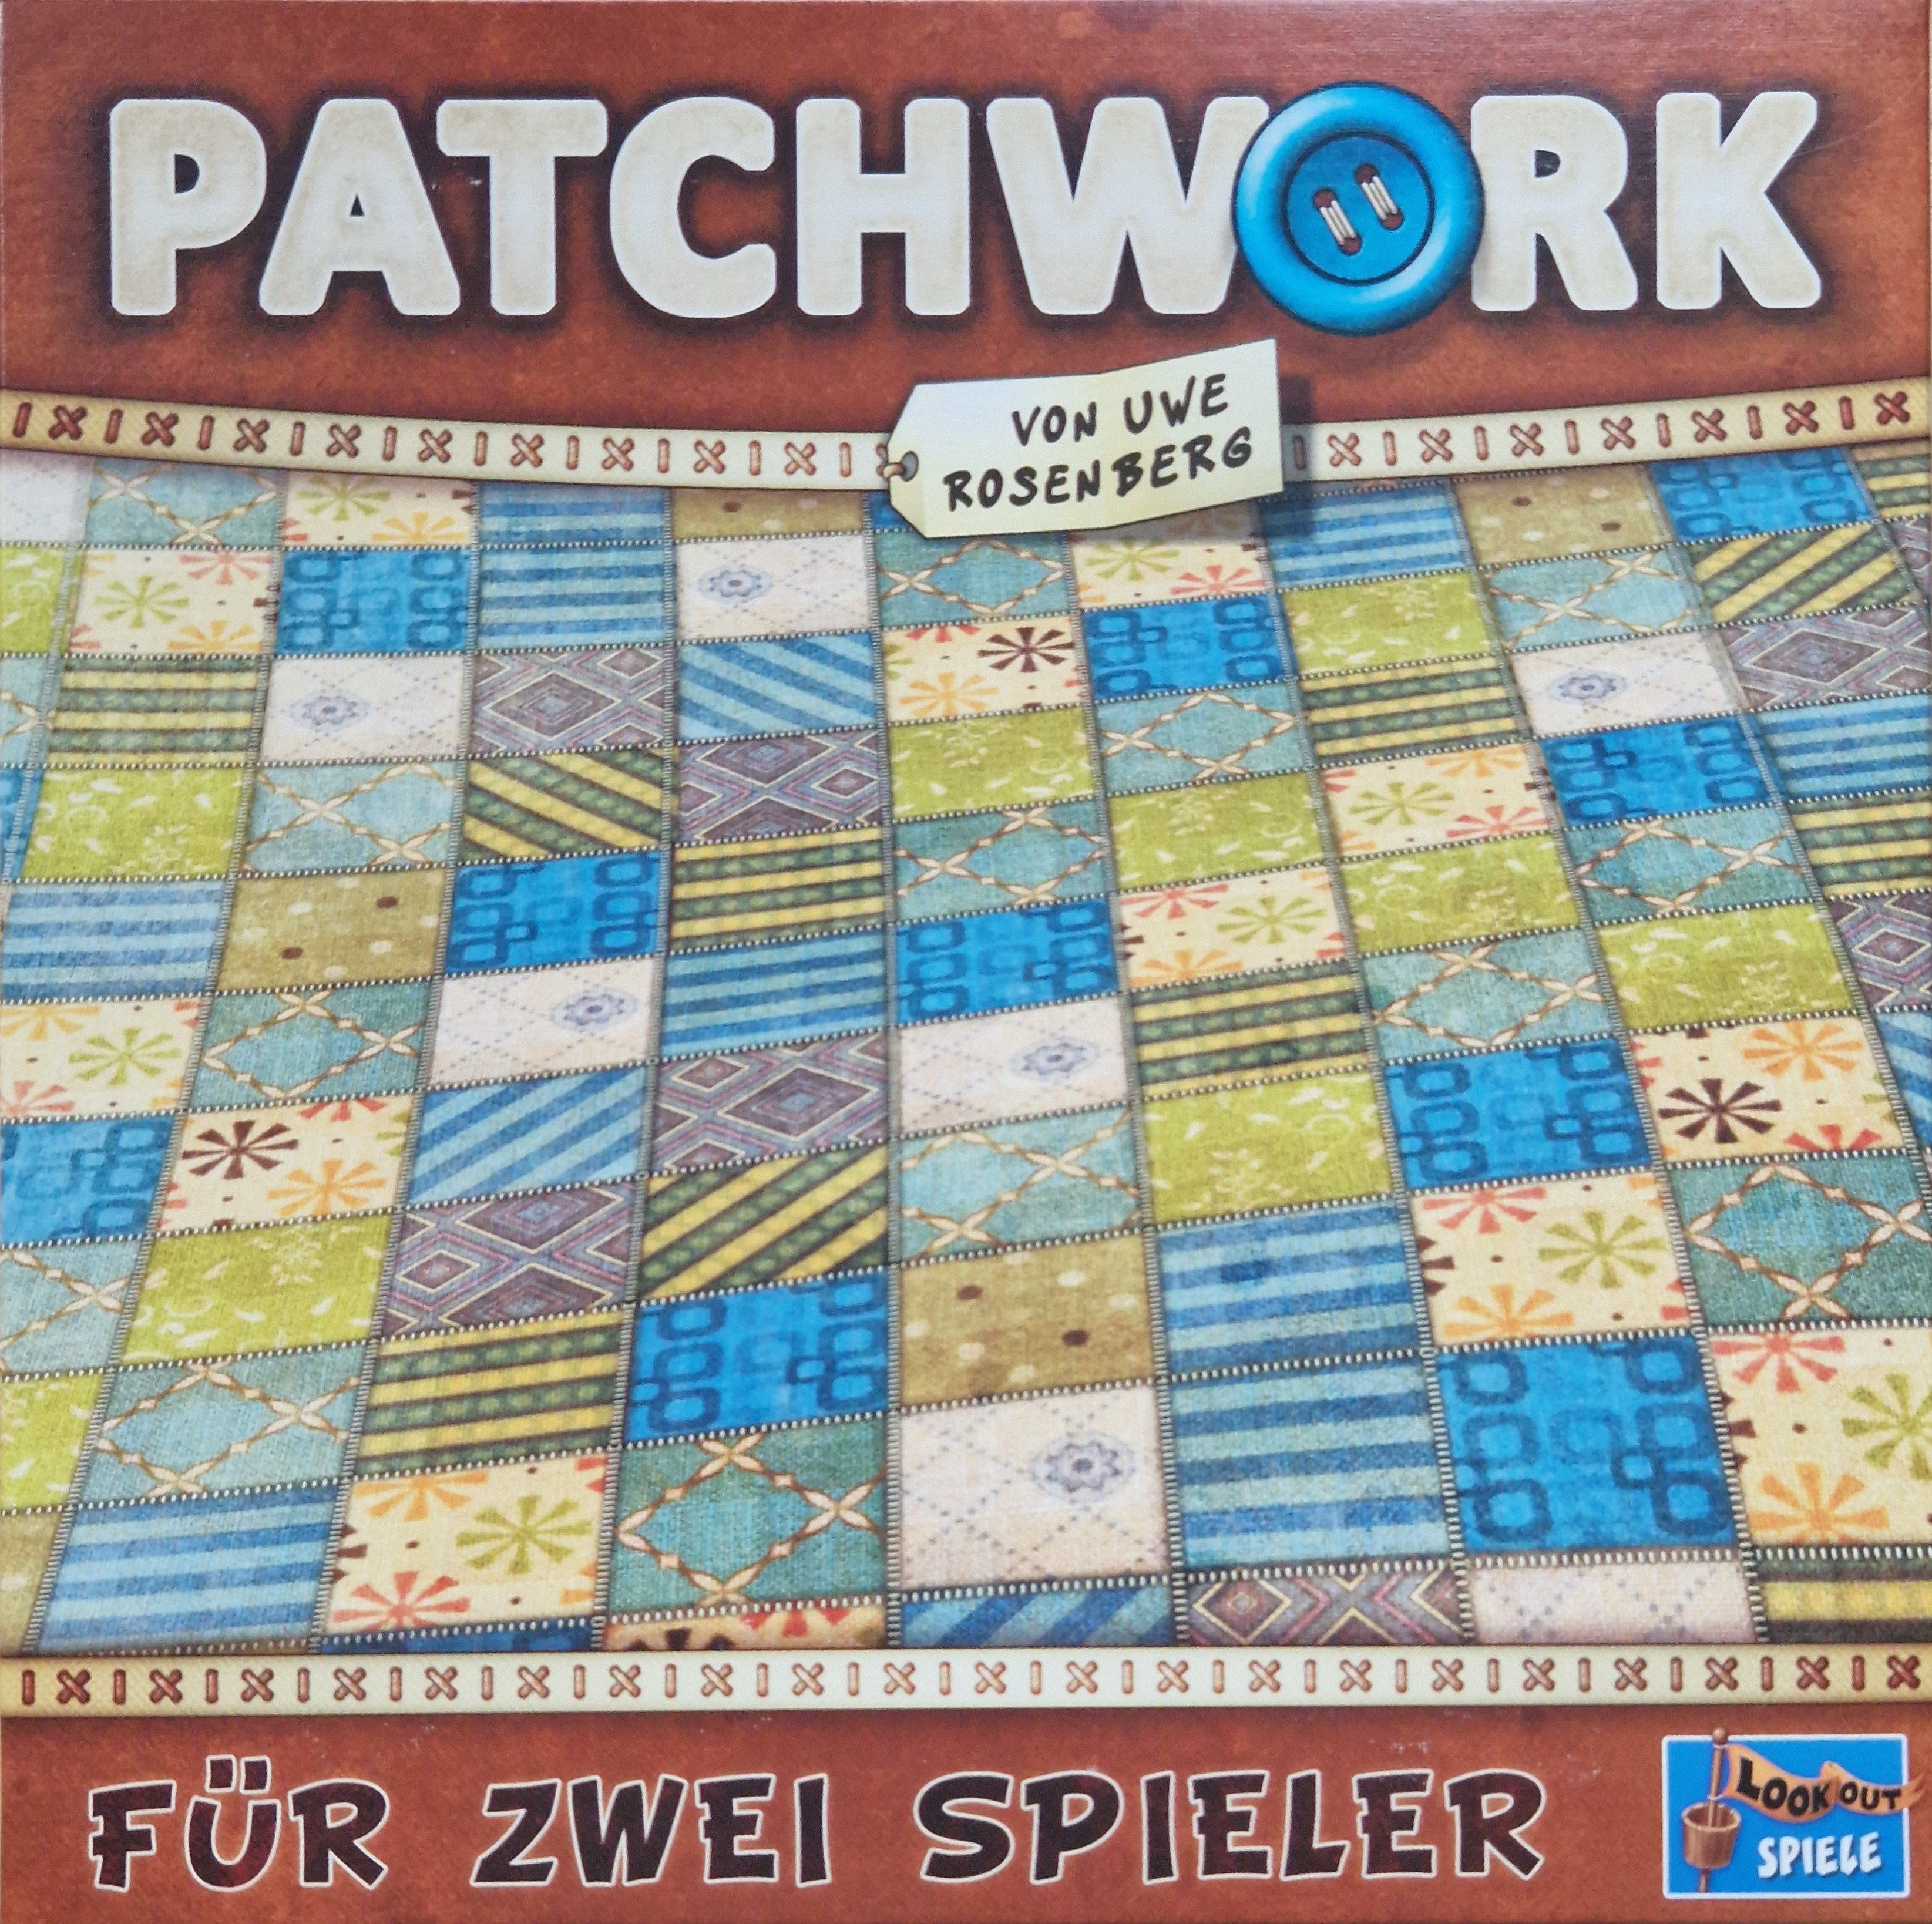
\includegraphics[width=0.28\textwidth]{res/pictures/assets/patchwork-cover.png}
    \caption[Cover von Patchwork]{\unskip}
    Cover von Patchwork
    \label{fig:patchwork-cover}
    \vspace*{-0.75cm}
\end{wrapfigure}

Patchwork ist ein Brettspiel von Uwe Rosenberg, das 2014 bei Lookout Spiele erschienen ist. Bei dem Brettspiel spielen zwei Spieler vom Alter 8 Jahre und aufwärts gegeneinander, wobei ein Spiel in der Regel ungefähr 30 Minuten lang ist \cite{LookoutSpielePatchwork}. Bei dem Brettspiel gestalten zwei Spieler jeweils eine eigne Decke aus Stoffresten, Flicken und Knöpfen, der Technik entsprechend, die der Titel vorgibt. \cite{SpielDesJahresPatchwork}

Das Ziel der Spieler ist mit den gegebenen Stoffplättchen unterschiedlicher Formen und Größen die vorgegebene Fläche zu füllen. Das Puzzlespiel erfordert taktisches Gespür, da die Flickenauswahl die Zugfolge und auch die Flickenauswahl des Gegenspielers beeinflusst. Immer können die Spieler jedoch nicht die gewünschten Flicken verwenden, da diese mit der Spielwährung Knöpfe aus der eigenen Kasse bezahlt werden müssen. An die begehrten Knöpfe kommen die Spieler über die bereits eingearbeiteten Flicken, welche Knöpfe auf sich abgebildet haben. Je mehr dieser Knöpfe auf der eigenen Decke abgebildet sind, desto höher das Einkommen an Knöpfen. Wer am Schluss des Spiels die meisten Knöpfe erwirtschaftet und seine Decke gut bestickt hat, gewinnt den Nähwettstreit. \cite{SpielDesJahresPatchwork}

\section{Spieltheorie}
\label{chapter:spieltheorie}

TODO:

\subsection{Spielbaum}

TODO: Spielbaum, Entscheidungsbaum

\subsection{Spielkomplexität}

TODO:

\begin{itemize}
    \item \textbf{Zustandsraum-Komplexität}: TODO:
    \item \textbf{Spielbaumgröße}: TODO:
    \item \textbf{Entscheidungskomplexität}: TODO: needed?
    \item \textbf{Spielbaumkomplexität}: TODO:
\end{itemize}

\section{Lineare Programmierung}
\label{chapter:lineare-programmierung}

TODO:

\section{Minimax-Algorithmus}
\label{chapter:minimax-algorithmus}

TODO:

Hier haben wir mehr

\section{Monte Carlo Tree Search}
\label{chapter:monte-carlo-tree-search}

\acf{MCTS} ist ein Suchalgorithmus, welcher verwendet wird, um in einem Spiel die beste Aktion zu finden. Dazu wird der Algorithmus während der Entscheidungszeit des Computerspielers ausgeführt. Innerhalb dieser Zeit wird schrittweise ein Suchbaum erstellt. Dabei wird für jede Aktion eine Heuristik erstellt, indem sehr viele Spiele zufällig bis zum Ende ausgespielt werden. Dadurch ergibt sich über die Zeit eine Wahrscheinlichkeit für das Ergebnis des Spiels für jede mögliche Aktion \cite[S. 61]{2008.ParallelMCTS}. Der \ac{MCTS}-Suchprozess besteht aus vier Phasen:

\begin{enumerate}
    \item \textbf{Selektion}: Der Suchbaum wird beginnend ab dem Wurzelknoten bis zu einem Blattknoten durchlaufen, indem in jeder Ebene immer genau ein Kindknoten nach einer bestimmten Richtlinie ausgewählt wird. \cite[S. 187]{2018.ReinforcementLearning}
    \item \textbf{Expansion}: Der ausgewählte Blattknoten wird um ein weiteres Kind erweitert, indem ein noch nicht erforschte Aktion ausgeführt wird. \cite[S. 61]{2008.ParallelMCTS}
    \item \textbf{Simulation}: Ausgehend vom neu hinzugefügten Knoten wird das Spiel bis zum Ende simuliert, indem bis Spielende zufällige Aktionen ausgeführt werden. \cite[S. 61]{2008.ParallelMCTS}
    \item \textbf{Backpropagation}: Das Ergebnis der Simulation wird durch den Suchbaum rückpropagiert, indem das Ergebnis (Gewonnen oder Verloren) ausgehend von dem in Zweitens neu hinzugefügten Knoten bis zum Wurzelknoten hochgereicht wird. \cite[S. 187]{2018.ReinforcementLearning}
\end{enumerate}

Die vier Phasen sind anschaulich in Abbildung \ref{fig:mcts-phases} dargestellt. Diese Phasen werden so lange wiederholt, bis die Entscheidungszeit vorbei ist.

\begin{figure}[!ht]
    \centering
    
\includegraphics[width=\textwidth]{res/pictures/mcts-phases.pdf}
    \caption{Phasen des \acs{MCTS} Algorithmus}
    \label{fig:mcts-phases}
\end{figure}

Für die erste Phase der Selektion wird im Normalfall die in \ref{eqn:uct} dargestellte \ac{UCT} Formel verwendet. Die \ac{UCT} Formel balanciert die Entscheidung zwischen der Ausnutzung von bereits bekannten Aktionen mit der Erkundung von unsicheren Aktionen \cite[S. 206]{2009.ComputerGoMCTS}. Dazu wird im ersten Teil die Anzahl der Siege ($w$) durch die Anzahl der Besuche des Kindknotens ($n$) geteilt. Dieser Term wird immer größer, je öfters eine Simulation nach einem Knotenbesuch gewonnen wird. Der andere Term wird immer größer, je weniger ein Knoten im Vergleich zu seinem Elternknoten ($N$) besucht wird und erzwingt somit auch die Erkundung weniger besuchter Knoten. Bei $c$ handelt es sich um eine Erkundungskonstante, welche das Verhältnis zwischen Ausnutzung und Exploration regelt und normalerweise auf $\sqrt{2}$ gesetzt wird.

\begin{equation}
    \label{eqn:uct}
    \mathbb{U}\mathbb{C}\mathbb{T} = \frac{w}{n} + c \cdot \sqrt{\frac{\ln N}{n}}
\end{equation}

Ein entscheidender Vorteil von \ac{MCTS} ist, dass keine statische Evaluierungsfunktion einer Position wie bei vergleichbaren Algorithmen existieren muss \cite[S. 61]{2008.ParallelMCTS}, da durch zufällige Erkundungen eines Teils des Suchbaums eine Approximation für den tatsächlichen Wert geschaffen wird. \ac{MCTS} hat sich vor allem für Spiele mit einer sehr großen Anzahl an Aktionen bzw. möglichen Zuständen als besser geeignet als traditionelle \hyperref[chapter:minimax-algorithmus]{Minimax}-basierte Programme herausgestellt \cite[S. 1]{2013.MCTSAndMinimaxHybrids} und ist aus diesem Grund auch zu großen Teilen für die Verbesserung der Computergegner in solchen Spielen wie beispielsweise Go verantwortlich \cite[S. 2006]{2009.ComputerGoMCTS} \cite[S. 185]{2018.ReinforcementLearning}.

\section{AlphaZero}
\label{chapter:alphazero}

TODO:

\section{Interaktive Systeme}
\label{chapter:interaktive-systeme}

Ein System ist die Gesamtheit von Elementen, die aufeinander bezogen und miteinander verbunden sind und auf eine Weise interagieren, dass sie als eine aufgaben-, sinn-, oder zweckgebundene Einheit angesehen werden können \cite{2014.Systeme}. Interaktiv ist ein solches System, wenn der Benutzer durch seine Bedienhandlungen den Arbeitsablauf des Systems beeinflussen kann \cite[S. 3]{2011.Heinecke}.

Beispiele für interaktive Systeme neben Flugzeugen und Kaffeeautomaten auch Softwareprodukte, die auf Benutzereingaben reagieren, wie das in dieser Studienarbeit entstehende Computerspiel auf der Grundlage von Patchwork. Um dem Benutzer die bestmögliche Erfahrung im Umgang mit dieser Software zu gewährleisten, werden im Folgenden einige Konzepte und Forschungen aus dem Bereich der interaktiven Systeme erläutert, die im Computerspiel Gebrauch finden sollen.

\subsection{Gestaltgesetze}
Die visuelle Wahrnehmung wird deutlich durch Gestaltgesetze oder Gestaltprinzipen beeinflusst. Insgesamt wurden 100 Gestaltgesetzte zur Anordnung von Information sowie zur Wahl von Farben und Formen von Max Wertheimer nach umfangreichen Untersuchungen und Analyse aufgestellt. Die Beachtung der Gesetze liefern eine Verbesserung der Wahrnehmbarkeit, eine Erleichterung des Suchens und Erkennens von Objekten oder Daten und der Vermeidung von fälschlicherweise wahrgenommenen Zusammenhängen. \cite[S. 55 f.]{2010.Preim} Im Folgenden sind einige Gesetze aufgelistet, die in der Studienarbeit Anwendung finden sollen:

\begin{itemize}
\item \textbf{Gesetz der Nähe}: Räumliche Nähe von Objekten führt dazu, dass sie als zusammengehörig wahrgenommen, selbst wenn Farbe und Form sich unterscheiden. Als Konsequenz hieraus sollten Unterschiede durch große Distanz vermittelt werden. \cite[S. 56]{2010.Preim}
\item \textbf{Gesetz der Gleichheit}: Eine Gleichheit von Form und Farbe führt, wie das Gesetz der Nähe, jedoch in geringerem Maße zu einer Wahrnehmung der Zusammengehörigkeit. \cite[S. 56]{2010.Preim}
\item \textbf{Gesetz der Prägnanz}: Objekte, die sich von anderen durch bestimmte Merkmale abheben, werden bevorzugt wahrgenommen. Jedes Objekt wird so wahrgenommen, dass es in einer möglichst einfachen geometrischen Struktur resultiert. \cite{Gestaltgesetze}
\item \textbf{Gesetz der Ähnlichkeit oder Gleichheit}: Einander ähnliche Objekte werden eher als zusammengehörig erlebt, als Objekte, die einander unähnlich sind. Je stärker die Ähnlichkeit , desto zusammengehöriger wirken die Objekte. \cite{Gestaltgesetze}
\item \textbf{Gesetz der gemeinsamen Bewegung}: Zwei oder mehrere sich gleichzeitig in eine Richtung bewegende Objekte werden meist als eine Einheit oder Gestalt wahrgenommen. \cite{Gestaltgesetze}
\item \textbf{Gesetz der Gleichzeitigkeit}: Objekte, die sich zur gleichzeitig verändern werden meist als zusammengehörig empfunden. \cite{Gestaltgesetze}
\end{itemize}

\subsection{Wahrnehmung von Bewegung}

Die Fähigkeit des Menschen Bewegungen wahrzunehmen und vorherzusagen, ist sehr gut entwickelt. Der Mensch nimmt Bewegungen in seinem gesamten visuellen Feld, also auch in der Peripherie, präattentiv war. Aufgrund dieser Umstände sind Bewegungen zur Aufmerksamkeitslenkung besonders gut geeignet, müssen aber mit Bedacht eingesetzt werden, da abrupte Änderung, wie zum Beispiel das Blinken eines Icons, durch die aufmerksamkeitslenkende Wirkung vom Betrachter nicht ignoriert werden kann und störend wirken können. Trotzdem können Betrachter bis zu fünf gleichzeitig stattfindende Bewegungen korrekt interpretieren und dementsprechend reagieren, wobei die Geschwindigkeit und Komplexität der Bewegung einen Einfluss auf die Schwierigkeit haben. \cite[S. 60 f.]{2010.Preim}

\subsection{Konzepte bei der Gestaltung von Bedienelementen}
\textbf{Affordances} sind die wahrgenommenen Eigenschaften eines Geräts oder Software, die den Eindruck vermitteln, dass sie vom Benutzer bedient werden können. Die äußere Form eines Objektes legt die Bedienung nahe: Knöpfe können gedrückt werden, Hebel können in die eine und die andere Richtung bewegt werden und eine Liste von Einträgen zu Auswahl verwendet werden. Es wird zwischen realen und wahrnehmbaren Affordances unterschieden. Es wird von einer realen Affordance gesprochen, wenn der Benutzer diese als bedienbar erkennt, sie objektiv vorhanden ist und benutzt werden kann. Erkennt der Benutzer darüber hinaus andere Affordances (wahrnehmbare Affordances), die allerdings nicht intendiert oder existent sind, wird von falschen Affordances gesprochen. Diese falschen Affordances legen eine unkorrekte Bedienung nahe, die eventuell zur Fehlfunktion oder Zerstörung des Gegenstands führen können. Das Ziel eines jeden Designers sollte daher die Übereinstimmung der wahrnehmbaren und realen Affordances sein. Ebenso sollten versteckte Affordances, also real Affordances, die vom Benutzer nicht erkannt werden, vermieden werden. \cite[S. 136 ff.]{2010.Preim}

\textbf{Constraints} sind die sinnvolle Einschränkung der Freiheitsgrade des Benutzers zur korrekten Nutzung von Geräten oder Software. Eine falsche Bedienung soll so erschwert oder ausgeschlossen werden. Ein Beispiel für umgesetzte Constraints sind Steckverbindungen von Kabeln, welche nur auf eine Weise ineinanderpassen, während ein Negativbeispiel Zapfpistolen und Tanköffnungen sind, welche eine folgenreiche falsche Betankung mit dem falschen Kraftstoff eines Fahrzeugs ermöglichen. \cite[S. 136 ff.]{2010.Preim}

Ein \textbf{konzeptuelles Modell} oder \textbf{mentales Modell} beschreibt die Vorstellung, wie sich ein Gerät oder Software verhält, wenn der Benutzer mit diesem interagiert. Dieses Modell sollte die Bedienung des Geräts oder Software möglichst klar vermitteln. Hier spielen Abbildungen, welche den internen Zustand eines Systems nach außen an den Benutzer widerspiegeln, eine wichtige Rolle. Das Ziel ist natürliche Abbildungen zu entwickeln, die dem Benutzer bereits bekannt sind und weit verbreitete Analogien abbilden, wie zum Beispiel die Verwendung der Farbe Rot zur Gefahrenanzeige oder Warnung. Die Bedienung eines Geräts oder einer Software wird dann als intuitiv bezeichnet, wenn gute direkte Abbildungen existieren. Neben der Sichtbarkeit des Systemzustands ist die Vermittlung der möglichen Bedienhandlungen für das konzeptuelle Modell des Benutzers wichtig. Rückkopplungen an den Benutzer beschreiben, wie ein System auf Bedienhandlungen reagiert, wie schnell es zu einer Reaktion des Systems kommt und wie der Benutzer diese Reaktion wahrnehmen und interpretieren kann. \cite[S. 136 ff.]{2010.Preim}

\subsection{Direkte Manipulation mit Drag-and-Drop}
Bei der direkten Manipulation wird eine grafische Darstellung des zu bearbeitenden Objektes mit einem Zeigegerät manipuliert, woraufhin die Veränderung des Objektes sofort auf dem Bildschirm zu erkennen ist. Vorbild für diese Interaktionsform ist das physische Zeigen und Bewegen, welches entsprechende Kommandos aktiviert. Das interaktive System liefert dem Benutzer unmittelbar darauf eine klar erkennbare Rückkopplung, die zum Beispiel durch Hervorhebung des selektierten Objektes geschieht. Die direktmanipulative Handhabung orientiert sich an den natürlich gegebenen Fähigkeiten und Fertigkeiten des Benutzers. Erfolgreich ist dies Interaktionsform, wenn die Affordances korrekt wahrgenommen werden. \cite[S. 351]{2010.Preim}

Die direkte Manipulation mit Drag-und-Drop geht auf Jeff Raskin zurück beschreibt die Bewegung von Objekten auf einem grafischen Bildschirm mittels folgenden Mechanismus \cite[S. 184]{2010.Preim}:
\begin{enumerate}
\item Selektieren des Objektes am Ausgangspunkt \cite[S. 184]{2010.Preim}
\item Bewegung des Objektes mit gedrückter Maustaste \cite[S. 184]{2010.Preim}
\item Fallenlassen des Objektes am Ziel durch Loslassen des Maustaste \cite[S. 184]{2010.Preim}
\end{enumerate}
Dieser Mechanismus ermöglicht dem Benutzer Objekten intuitiv hin- und herzubewegen \cite[S. 129]{2010.Preim}.

